(i)The data is already continuous. The histogram is created using the following python code\\
\begin{lstlisting}
./solutions/20-10/stat/codes/exer41.py
\end{lstlisting}
The histogram is shown in figure \ref{fig:hist41_py}
\begin{figure}[!ht]
\centering
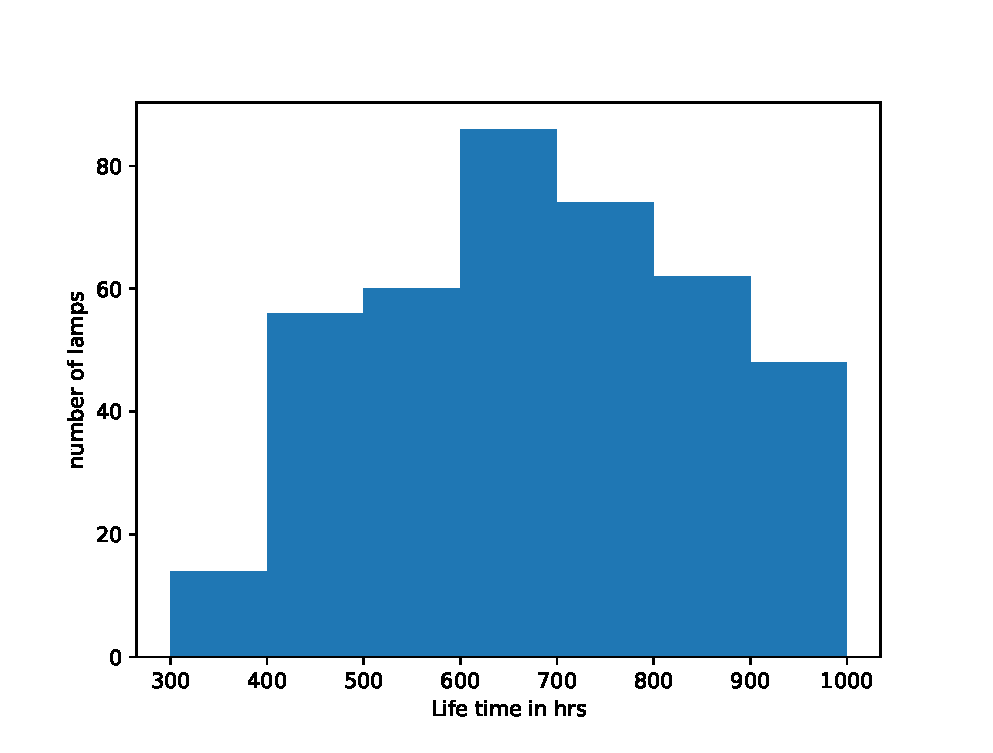
\includegraphics[width=\columnwidth]{./solutions/20-10/stat/codes/pyfigs/exer41.eps}
\caption{Lives of neon lamps}
\label{fig:hist41_py}
\end{figure}
(ii)184 lamps have a life time of more than 700 hours.
